\documentclass{neu_handout}
\usepackage{url}
\usepackage{amssymb}
\usepackage{amsmath}
\usepackage{marvosym}
\usepackage{graphicx}
\usepackage[pdftex]{graphicx}
\usepackage{subfigure}
\graphicspath{ {images/} }
\everymath{\displaystyle}


% Professor/Course information
\title{Homework 1 - Part 3}
\author{Emily Dutile}
\date{January 2018}
\course{CS7295}{Info Viz}

\begin{document}


\section*{Who is CS7295}

\subsection*{2. Data Types}

\begin{center}
Table 1: Data Types
\end{center}
\begin{center} 
\begin{tabular}[h]{l l l l}
\textbf{Column} & \textbf{Data Type} \\
City & categorical \\
Country & categorical \\ 
State & categorical \\
Native language & categorical \\
Languages known other than English & categorical \\
Preferred OS & categorical \\
Mobile OS & categorical \\
Favorite language & categorical \\
Chocolate or Vanilla & categorical \\
Preferred OS & categorical \\
Color & categorical \\
Favorite number & categorical \\
Temperate & quantitative \\
Amount of coffee & quantitative \\
Wake up & quantitative \\
To bed & quantitative \\
Visual encoding & quantitative
\end{tabular}
\end{center}

\subsection*{4. Data Clean-Up}
To clean up the data, the data was exported to a new excel spreadsheet. Column names were shortened for readability, categorical data was made the same (i.e.: USA vs. United States), null values were filled with None or NA, verbose answers were shorted, state abbreviations were spelled out, degrees were converted to Farenheight if necessary, exclamation points were removed, and numbers that were spelled out were many quantitative.\\

If this was a much larger data set, I would have wrote a web crawler in python using the BeautifulSoup library to extract the html and parse the desired text. Since there is no student name in the original dataset, joining would be difficult without a given key, so this step would be kept manual for sake of time.

\subsection*{6. Data Gathering}
From Piazza I compared the information hints as to what text blurb matched with the data in the csv. I simply inserted two rows for department (CCIS or other) and what degree program the individual is pursuing. There wasn't a great deal of cleaning the data here.

\subsection*{7. Questions}

\subsubsection*{7.1}
Is there a correlation between bedtime and coffee consumption? Please see Appendices for visual.\\

There seems to be a high correlation between individuals that go to bed around 1am and the amount of coffee consumed. Overall, it appears that individuals who go to bed earlier at night seem to consume less coffee.

\subsubsection*{7.2}
Is there a typical “profile” for someone who prefers to use a mobile phone with an
Android versus Apple OS?

\subsection*{8. Additional Questions and Visualizations}


\subsubsection*{8.1}
Is there a correlation between preferred programming language and preferred OS? Please see Appendices for visual.\\

@TODO - justify your choice of visual encoding and visualization design choices (i.e., marks, channels,
perceptual ordering, etc.

\subsubsection*{8.2}
What percentage of the class speaks another language if their native language is not English? Please see Appendices for visual.\\

@TODO - justify your choice of visual encoding and visualization design choices (i.e., marks, channels,
perceptual ordering, etc.

\subsubsection*{8.3}
Are students sleeping enough? Please see Appendices for visual.\\

\appendix
\section{Appendices}

\subsection*{7.1}
\begin{figure}[h]
\centering
{
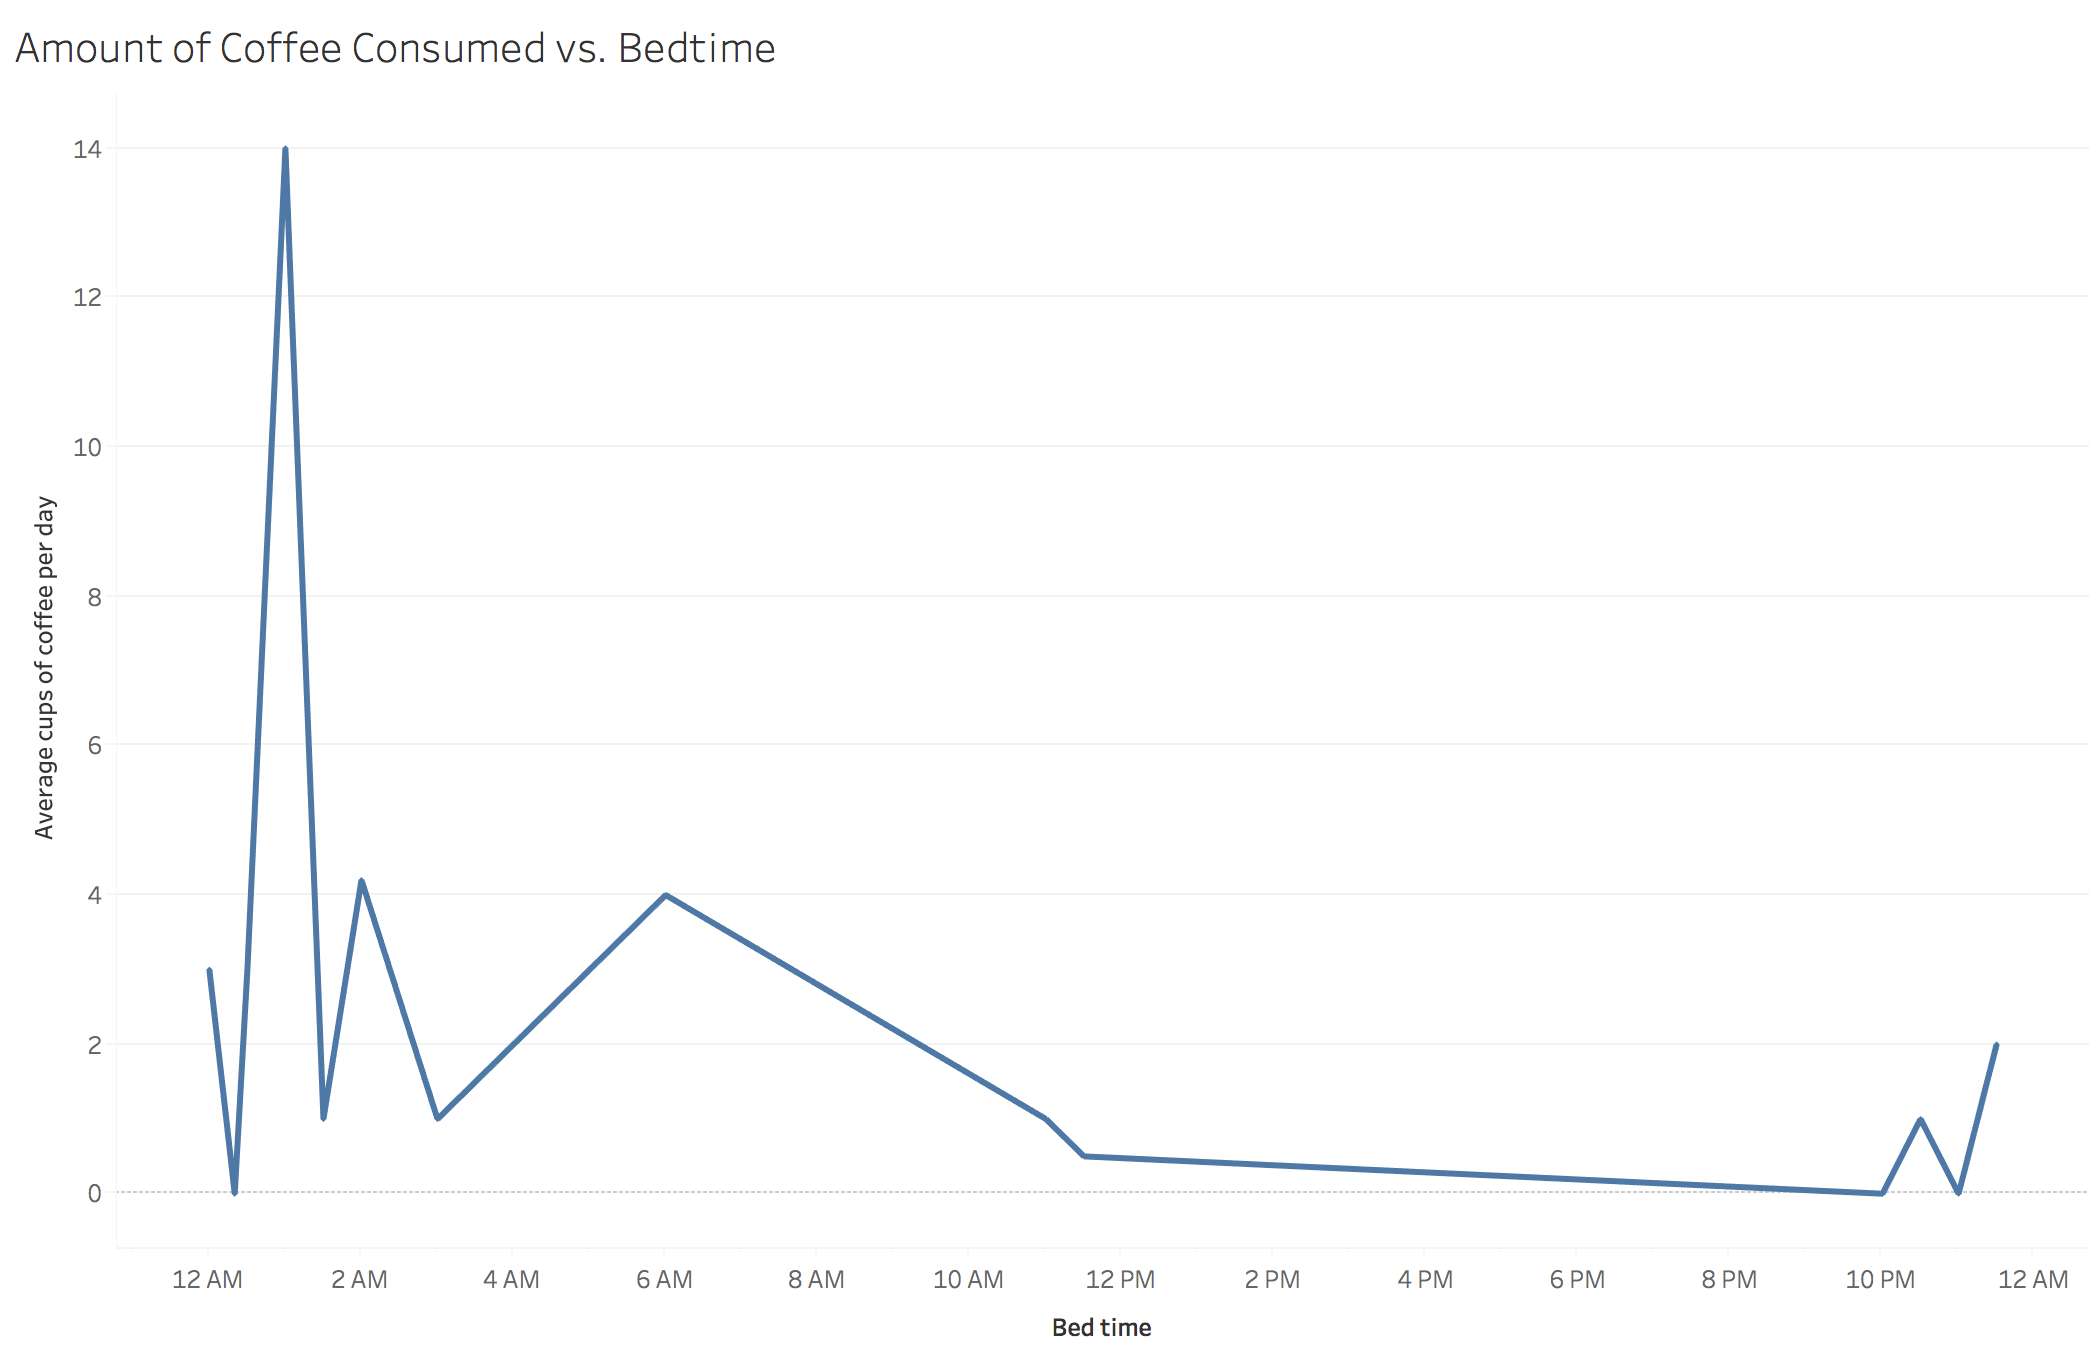
\includegraphics[width=0.7\linewidth]{bedtime_coffee}
}
\end{figure}


\end{document}
